\documentclass[12pt,a4paper]{article}

\usepackage[margin=1in]{geometry}
\usepackage[T1]{fontenc}
\usepackage{lmodern}
\usepackage{microtype}
\usepackage{graphicx}
\usepackage{float}
\usepackage{booktabs}
\usepackage{array}
\usepackage{enumitem}
\usepackage{hyperref}
\usepackage{xurl}
\usepackage{caption}
\usepackage{longtable}
\usepackage{amsmath}

\hypersetup{
  colorlinks=true,
  linkcolor=blue,
  urlcolor=blue,
  citecolor=blue
}
\setlength{\parskip}{0.45em}
\setlength{\parindent}{0pt}

\title{\textbf{GridShift TFT}\\
A Comparative Study of Time-Series Forecasting Under Solar-Related Grid Changes}
\author{Student Name(s) \\ Course / Section: [Insert] \\ Instructor: [Insert]}
\date{\today}

\begin{document}
\maketitle

\begin{abstract}
This report defines the problem, intended users, AI justification, data source, and planned preprocessing workflow for GridShift TFT. The project will compare Temporal Fusion Transformer (TFT), XGBoost, and Long Short-Term Memory (LSTM) models for hourly electricity-load forecasting using India's published electricity-demand, solar-generation, and wind-generation dataset. The proposed research question is whether model performance changes when later observations exhibit a demonstrable shift in load or renewable-generation patterns, and whether training-only synthetic time-series augmentation can improve robustness. This document describes the dataset and planned procedures; it does not claim experimental results before the downloaded files have been audited and processed.
\end{abstract}

\section{Phase 1: Problem Definition and AI Justification}

\subsection{Problem Statement}
Electricity-system operators must estimate future demand to support generation scheduling, reserve planning, and reliable grid operation. Forecasting becomes more challenging when the relationship between time, demand, and renewable generation changes. Solar output varies by time of day and weather, while demand also varies with season, temperature, and human activity. As renewable generation becomes a larger part of the electricity mix, historical load patterns may not remain stable.

GridShift TFT will study hourly electricity-load forecasting using load, solar-generation, and wind-generation observations. It will compare TFT, XGBoost, and LSTM under a chronological evaluation design. The project will specifically test whether later periods exhibit a measurable distribution or relationship shift; a later test period alone will not be described as a structural-shift experiment unless the data supports that conclusion.

The study is observational. Co-movement between solar generation and load does not, by itself, establish that solar adoption caused a change. Findings will be stated in terms of measured forecasting performance and documented data patterns.

\subsection{Target Audience}
The intended audience includes:
\begin{itemize}[leftmargin=*]
  \item \textbf{Grid and system-planning analysts:} people who use demand forecasts to support operational planning.
  \item \textbf{Renewable-energy researchers:} researchers studying how variable renewable generation relates to grid demand.
  \item \textbf{Machine-learning practitioners:} practitioners comparing sequence models and tree-based methods for time-series forecasting.
  \item \textbf{Academic evaluators:} readers interested in a reproducible comparison of forecasting accuracy and robustness.
\end{itemize}

The project is a research prototype, not a production grid-control system. It will not be used to dispatch power or make operational decisions.

\subsection{Research Question and Scope}
The primary research question is:
\begin{quote}
How do TFT, XGBoost, and LSTM compare in hourly electricity-load forecasting on India's grid-level data, and how does their performance change in a later period if a measurable shift in load or renewable-generation patterns is present?
\end{quote}

A secondary question is whether TimeGAN-generated training sequences, validated for realism and generated without access to the held-out test period, improve performance on the later period.

The study will report Mean Absolute Error (MAE) and Root Mean Squared Error (RMSE). Model comparisons will use the same target, chronological splits, forecast horizon, and information available at prediction time. The precise forecast horizon and feature set will be recorded after the raw workbook schema has been inspected.

\subsection{Why AI / Machine Learning Is Appropriate}
Rule-based methods can encode fixed assumptions, but electricity demand is affected by interacting temporal, weather-related, calendar, and generation patterns. Those relationships may be nonlinear and may change over time. Supervised learning provides a way to estimate such relationships from historical observations and assess generalization on later data.

The selected methods represent different modelling approaches:
\begin{itemize}[leftmargin=*]
  \item \textbf{XGBoost:} gradient-boosted decision trees that provide a strong tabular baseline when time-based, lagged, and renewable-generation features are engineered.
  \item \textbf{LSTM:} a recurrent neural network designed to learn sequential dependencies.
  \item \textbf{TFT:} a neural forecasting architecture designed for multi-horizon time-series prediction with variable selection and attention mechanisms.
\end{itemize}
The need for AI is therefore an empirical question as well as a modelling rationale: results must show whether these methods improve accuracy or robustness over simple baselines. The project should include a naive seasonal baseline (for example, the previous day's value at the same hour) if time permits, so the complex models are not compared only against one another.

\section{Phase 2: Data Acquisition and Preprocessing}

\subsection{Dataset Source and Provenance}
The selected dataset is:
\begin{quote}
Mukherjee, Debanjan; Kalita, Karuna; Kumar, Subhash (2025). \textit{Electricity Demand, Solar and Wind Generation Data (September 2021--June 2025) of India at 1-hour interval}. Mendeley Data, Version 2. DOI: \url{https://doi.org/10.17632/y58jknpgs8.2}.
\end{quote}

Dataset record: \url{https://data.mendeley.com/datasets/y58jknpgs8/2}.

The record states that the data was provided by North-Eastern Regional Load Despatch Centre, Grid-India, under India's Ministry of Power, and describes hourly PMU electricity-demand, solar-generation, and wind-generation data for the combined five regional grid networks. The record lists a CC BY 4.0 licence.

\textbf{Metadata discrepancy to verify:} the dataset title and file list indicate coverage through June 2025, and the file list includes a workbook named \texttt{January 2024- June 2025.xlsx}. However, the record's description text still states that the period is September 2021 to December 2023. The report will preserve this discrepancy rather than silently assume which statement is authoritative. Actual coverage will be verified from workbook contents and timestamps.

\subsection{Collection Procedure and Evidence}
The data will be acquired manually from the Mendeley Data record. The raw Excel files will be retained unchanged in \texttt{data/raw/}. The following evidence will be retained with the project:
\begin{itemize}[leftmargin=*]
  \item the dataset DOI and source URL listed above;
  \item downloaded original workbook filenames;
  \item the output of \texttt{audit\_india\_dataset.py}, which records sheet names, observed column headers, and sample rows;
  \item the generated \texttt{cleaning\_report.json}, containing row counts, missing-value summaries, outlier flags, and split sizes after processing.
\end{itemize}
No API call or web-scraping process is claimed. The acquisition method is a documented download from the dataset repository.

\subsection{Initial Data Audit}
Before transformation, the audit script will inspect every Excel workbook and report its sheets, columns, and sample records. This step is required because workbook header layouts and exact field names must be confirmed from the downloaded data, not inferred from the dataset title.

The following properties will be verified before modelling:
\begin{itemize}[leftmargin=*]
  \item actual timestamp fields and timezone conventions, if stated;
  \item units and meaning of the load, solar, and wind variables;
  \item whether records are national aggregates or contain separate regional observations;
  \item coverage gaps, duplicate timestamps, repeated header rows, and missing periods;
  \item whether the five regional networks are separately represented or already combined.
\end{itemize}

\subsection{Cleaning Implementation}
The provided Python cleaning script implements a configurable workflow. Exact column names and sheet/header settings must be populated from the audit output before running it. The script intentionally stops when required fields are not configured or when duplicate timestamps are found, rather than silently guessing or discarding potentially meaningful regional records.

The planned operations are:
\begin{enumerate}[leftmargin=*]
  \item \textbf{Empty records:} remove fully empty rows and columns.
  \item \textbf{Timestamp validation:} parse the configured timestamp column and report unparseable timestamps.
  \item \textbf{Numeric conversion:} convert the configured load and solar fields, and wind if present, to numeric values; non-numeric placeholders become missing values and are counted.
  \item \textbf{Duplicate handling:} detect repeated timestamps. If repetitions occur, inspect whether they represent regions or duplicated records. Regional observations must be handled with an explicit region key and a justified aggregation rule before deduplication.
  \item \textbf{Missing values:} interpolate only short internal gaps of at most two consecutive hourly records. Longer gaps remain missing. Rows without the target load after this limited interpolation are excluded from the forecasting table; all counts are reported.
  \item \textbf{Outlier screening:} flag observations outside the interquartile-range (IQR) bounds. Flags are retained for inspection; observations are not automatically deleted because extreme electricity demand can be real. Clipping is an optional configuration and should be justified before use.
  \item \textbf{Time features:} derive hour, day of week, and month from the timestamp, with sine/cosine encodings for cyclic calendar patterns.
  \item \textbf{Chronological split:} reserve the final 20\% of ordered observations for testing. The split is temporal, not random.
  \item \textbf{Scaling:} fit a standard scaler on training rows only and apply that fitted transformation to the test rows to avoid leakage.
\end{enumerate}

These operations are a proposed preprocessing policy, not a claim that the source dataset contains missing values, duplicates, or outliers. Actual counts will be inserted after execution.

\subsection{Feature Strategy}
The initial feature set will use verified load, solar-generation, and wind-generation columns, plus calendar features derived from the timestamp. After the schema is confirmed, lagged load and generation features may be added. Lag features must use only observations available before the forecast origin.

Continuous variables will be scaled for models that benefit from scaling. The script uses \texttt{StandardScaler} fitted on training data only. XGBoost generally does not require standardization of numerical features, so scaled and unscaled variants may be compared if time permits. The current script retains both original numeric columns and scaled copies.

The available dataset description does not establish that weather variables are included. Weather will not be claimed as a feature unless a verified source and aligned observations are added. Likewise, a solar-generation series alone does not directly measure installed solar capacity or household adoption.

\subsection{Exploratory Data Analysis}
The Python script saves the following figures from the selected raw series:
\begin{itemize}[leftmargin=*]
  \item \texttt{raw\_missingness.png}: proportion of missing observations in selected variables;
  \item \texttt{raw\_distributions.png}: histograms of selected numeric variables;
  \item \texttt{raw\_correlation.png}: pairwise correlations among numeric variables;
  \item \texttt{raw\_time\_series.png}: load and generation series over time.
\end{itemize}

Correlation is descriptive and will not be interpreted as evidence of causation. Figures will be included only after they have been generated from the downloaded files. No artificial plots or invented data summaries are included in this report.

\begin{figure}[H]
\centering
\IfFileExists{figures/raw_missingness.png}
  {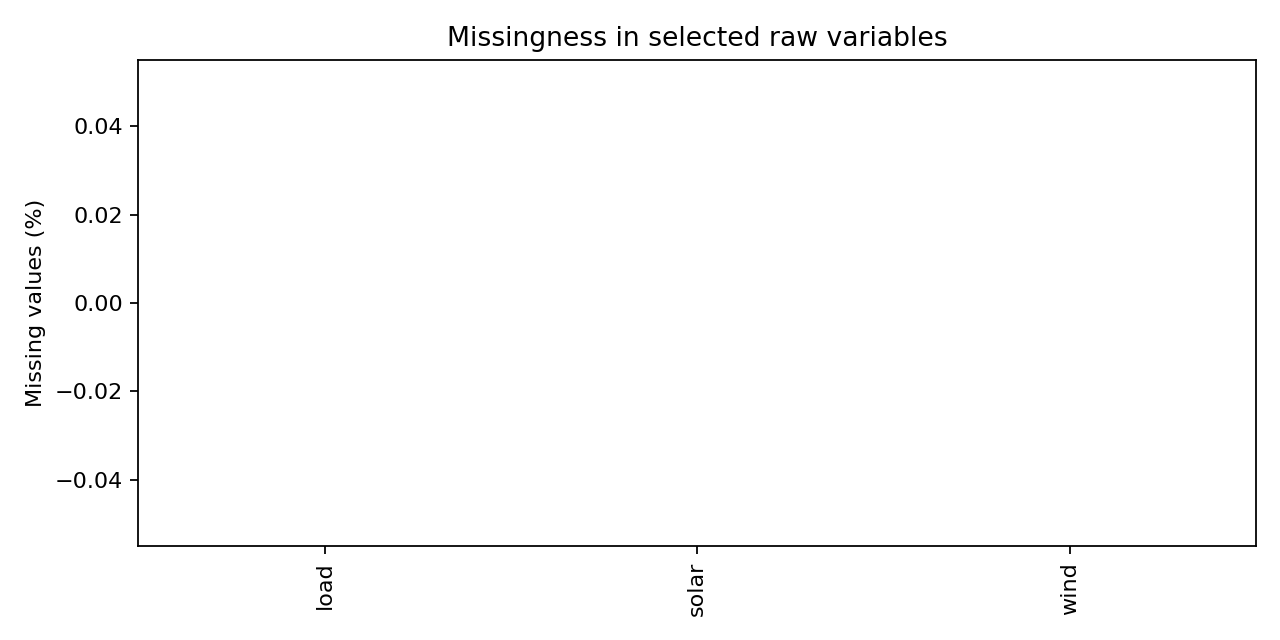
\includegraphics[width=0.78\linewidth]{figures/raw_missingness.png}}
  {\fbox{\parbox{0.75\linewidth}{\centering Run the preprocessing script and copy \texttt{raw\_missingness.png} into the \texttt{figures/} folder.}}}
\caption{Missingness in the selected raw variables. The figure will be generated from the downloaded dataset.}
\end{figure}

\begin{figure}[H]
\centering
\IfFileExists{figures/raw_distributions.png}
  {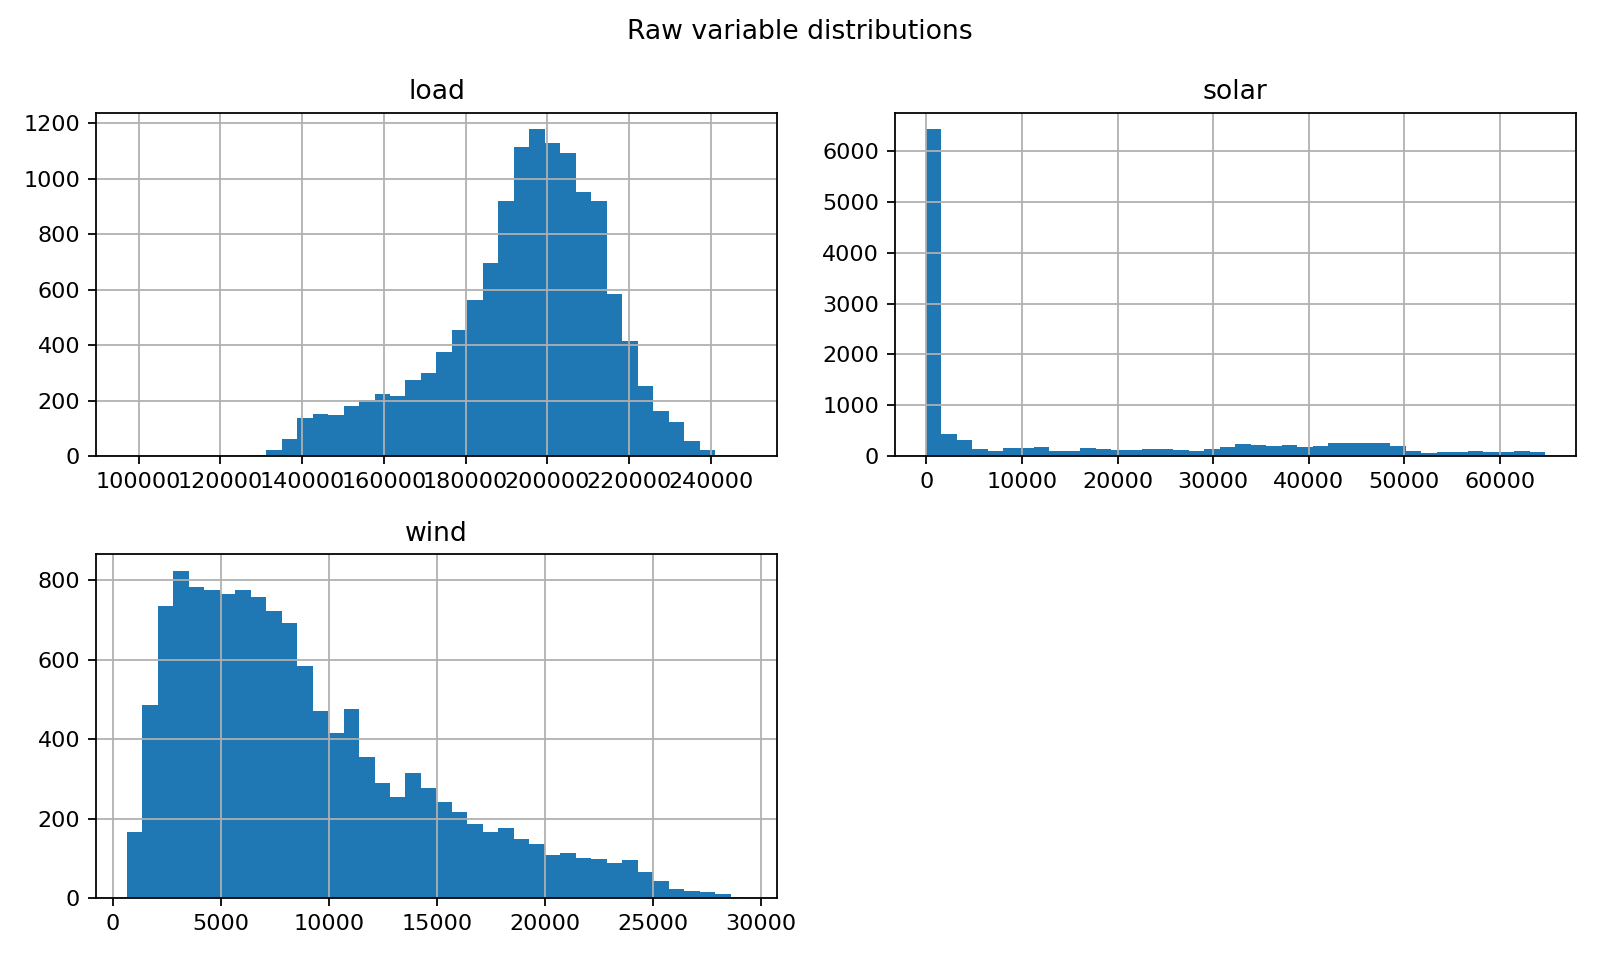
\includegraphics[width=0.92\linewidth]{figures/raw_distributions.png}}
  {\fbox{\parbox{0.75\linewidth}{\centering Run the preprocessing script and copy \texttt{raw\_distributions.png} into the \texttt{figures/} folder.}}}
\caption{Raw distributions of selected numeric variables.}
\end{figure}

\begin{figure}[H]
\centering
\IfFileExists{figures/raw_correlation.png}
  {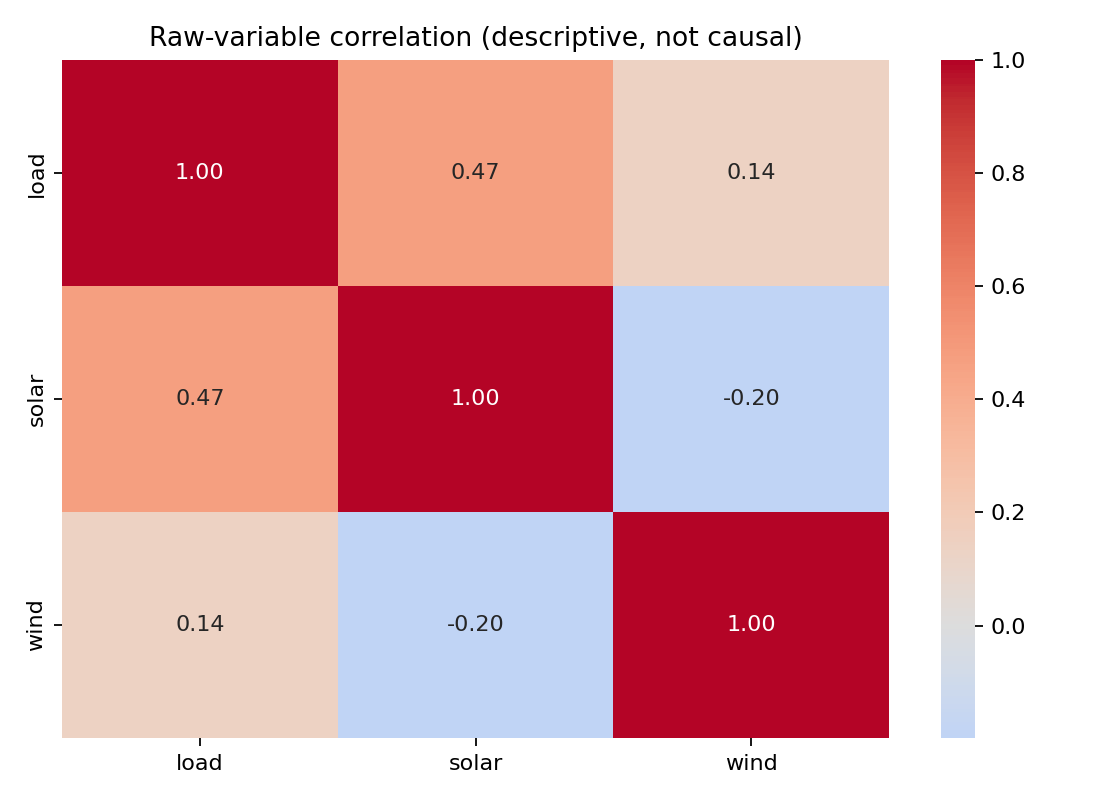
\includegraphics[width=0.78\linewidth]{figures/raw_correlation.png}}
  {\fbox{\parbox{0.75\linewidth}{\centering Run the preprocessing script and copy \texttt{raw\_correlation.png} into the \texttt{figures/} folder.}}}
\caption{Correlation among selected raw numeric variables. Correlation does not establish causation.}
\end{figure}

\begin{figure}[H]
\centering
\IfFileExists{figures/raw_time_series.png}
  {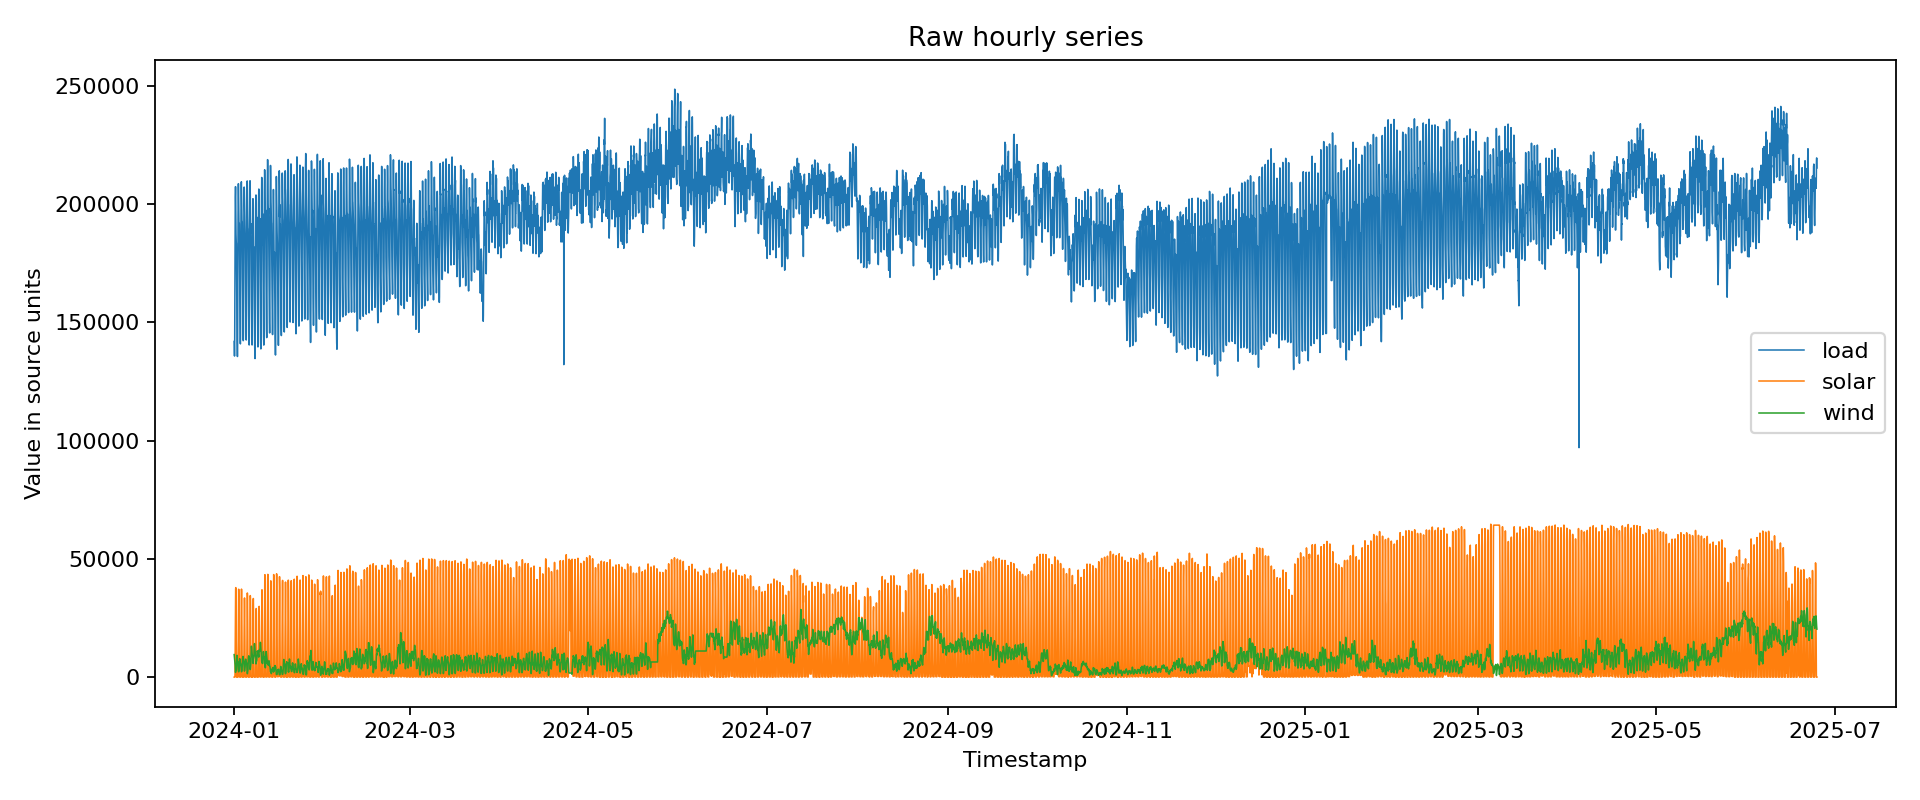
\includegraphics[width=0.95\linewidth]{figures/raw_time_series.png}}
  {\fbox{\parbox{0.75\linewidth}{\centering Run the preprocessing script and copy \texttt{raw\_time\_series.png} into the \texttt{figures/} folder.}}}
\caption{Hourly load and renewable-generation series.}
\end{figure}

\subsection{Reproducibility and Leakage Prevention}
The raw files will be preserved separately from processed files. The audit JSON and cleaning JSON will record observed columns, source filenames, missing-value counts, outlier flags, and train/test sizes. All splits will be chronological. Any TimeGAN model used in a later phase will be fitted only on the training partition; the held-out test period will not be used to generate synthetic training examples or tune model settings.

\section{Current Status and Items Requiring Verification}
At the time this template was prepared, the dataset repository and citation were checked, but the Excel workbook contents had not yet been audited in this report. Therefore, the following remain to be completed after download and execution:
\begin{itemize}[leftmargin=*]
  \item confirm sheet names, headers, units, timestamps, and aggregation level;
  \item confirm the actual coverage and resolve the repository metadata discrepancy using file contents and, if necessary, repository clarification;
  \item run the scripts and insert observed row counts and cleaning statistics;
  \item insert EDA figures generated from the actual files;
  \item document any manual header/format adaptations and justify missing-value/outlier decisions.
\end{itemize}

\section{References}
\begin{enumerate}[leftmargin=*]
  \item Mukherjee, D., Kalita, K., \& Kumar, S. (2025). \textit{Electricity Demand, Solar and Wind Generation Data (September 2021--June 2025) of India at 1-hour interval} (Version 2). Mendeley Data. \url{https://doi.org/10.17632/y58jknpgs8.2}.
  \item Mendeley Data. Dataset record and downloadable files. \url{https://data.mendeley.com/datasets/y58jknpgs8/2}.
  \item Chen, T., \& Guestrin, C. (2016). XGBoost: A Scalable Tree Boosting System. In \textit{Proceedings of the 22nd ACM SIGKDD International Conference on Knowledge Discovery and Data Mining}. \url{https://doi.org/10.1145/2939672.2939785}.
  \item Hochreiter, S., \& Schmidhuber, J. (1997). Long Short-Term Memory. \textit{Neural Computation, 9}(8), 1735--1780. \url{https://doi.org/10.1162/neco.1997.9.8.1735}.
  \item Lim, B., Arik, S. O., Loeff, N., \& Pfister, T. (2021). Temporal Fusion Transformers for Interpretable Multi-horizon Time Series Forecasting. \textit{International Journal of Forecasting, 37}(4), 1748--1764. \url{https://doi.org/10.1016/j.ijforecast.2021.03.012}.
  \item Yoon, J., Jarrett, D., \& van der Schaar, M. (2019). Time-series Generative Adversarial Networks. In \textit{Advances in Neural Information Processing Systems}. \url{https://papers.nips.cc/paper/2019/hash/c9efe5f26cd17ba6216bbe2a7d26d490-Abstract.html}.
\end{enumerate}

\end{document}
